\documentclass[a4paper, 11pt]{article}
\usepackage[utf8]{inputenc}
\usepackage[polish]{babel}
\usepackage[MeX]{polski}
\usepackage[T1]{fontenc}
\usepackage{geometry}
\usepackage{fancyhdr}
\usepackage{graphicx}
\frenchspacing %wyłączenie dłuższych spacji na końcu każdego zdania.

\geometry{a4paper,tmargin=2.5 cm,bmargin=1.5cm,lmargin=2cm,rmargin=2cm}
\setlength{\headheight}{11pt} %przesuwa calosc w dol
\setlength{\headsep}{0.5cm} %przesuwa zawartosc wraz z dolna stopka w dol (bez gornej stopki
\setlength{\footskip}{1.2cm} %przesuwa w dol stopke od bmargin - konca tekstu

\newcommand{\przedmiot}{Indywidualny Projekt Programistyczny}
\newcommand{\podpisAutora}{Rafał Soszyński, nr indeksu 335786}
\newcommand{\data}{\today}%zamienić jeśli inaczej

\newcommand*{\naglowek}{
\begin{center}
{\huge \underline{\przedmiot}}
\\\vspace{0.50cm}
%% Koniecznie uzupełnić numer
Opis projektu: Gra planszowa typu RPG
\\\vspace{0.1cm}
{\large \textbf{\podpisAutora}}
\\\vspace{0.15cm}
\small{\data}
\\\vspace{1cm}
\end{center}
}

\begin{document}
\naglowek

\noindent\textbf{Zasady gry:}

Jest to gra typu RPG, gdzie każdy gracz posiada własną postać z określonymi statystykami i ekwipunkiem, którą rozwija przez całą rozgrywkę.
Gracz wybiera jaką klasą (np. łowca, mag) oraz klasą (np. elf, człowiek) będzie grał (ma to m.in. wpływ na statystykę oraz ekwipunek).
Gracze poruszają się systemem turowym po planszy złożonej z hexów.
Każde pole ma określony rodzaj (np. las, góra droga), co wpływa na możliwość wykonania ruchu.
Niektóre z pól są wyszczególnione i na nich odbywają się walki z przygotowanymi przeciwnikami.
Walka skłąda się z naprzemiennych ataków lub działań specjalnych (jak użycie przedmiotu).
Są też pola-miasta gdzie gracz może podjąć się jakiegoś zadania (typu przynieś, zbierz, zabij, itp.), handlować ekwipunkiem czy uleczyć swoją postać.
Na wspomniany ekwipunek składają się pancerz, broń, mikstury oraz artefakty.
Gra kończy się w przypadku, gdy jeden z graczy osiągnie określony poziom i wykona pewne trudne zadanie (ze specjalnej puli).

\vspace{0,5cm}

\noindent\textbf{Opis modułów programu:}

\begin{itemize}
	\item \underline{Okno Nowej Gry}: Wyświetla okno pozwalające wprowadzić ustawienia początkowe rozgrywki.
	
	\item \underline{Cykl Gry}: Zarządza przebiegiem gry. Określa aktualnego gracza oraz moment gry.
	
	\item \underline{Plansza}: Trzyma informacje o układzie planszy, udostępnia listę możliwych ruchów dla gracza.
	
	\item \underline{Parser Układu}: Pobiera z dysku ustawienie planszy.
	
	\item \underline{Obszar Planszy}: Odpowiada za wyświetlanie hexów na ekranie i wodotryski. Udostępnia wyświetlenie konkretnego ruchu gracza.
	
	\item \underline{Mistrz Gry}: Odpowiada za wyznaczanie możliwych akcji gracza oraz nadzorowanie walk. Dodatkowo prosi o wyświetlenie komponenty graficzne (poza Obszarem Planszy, za który odpowiada Plansza), a także w razie potrzeby odbiera od nich "wyklikane" informacje. Udostępnia informacje o graczu.
	
	\item \underline{ParserKart}: Pobiera z dysku bazę zadań, przedmiotów i przeciwników oraz przekazuje ją Mistrzowi Gry.
	
	\item \underline{Panel Akcji}: Wyświetla na rządanie listę akcji i informuje o ewentualnym wyborze.
	
	\item \underline{Okno Gracza}: Wyświetla obecne dane gracza. Pozwala na wyświetlenie Ekwipunku i Zadań.
	
	\item \underline{Ekwipunek}: Wyświetla i pozwala zarządzać ekwipunkiem gracza.
	
	\item \underline{Zadania}: Wyświetla i pozwala zarządzać podjętymi zadaniami gracza. 
	
	\item \underline{Tawerna}: Wyświetla okno tawerny (miejsca w mieście, gdzie gracz może podjąć się nowych zadań).

	\item \underline{Bazar}: Wyświetla okno bazaru (miejsca w mieście, gdzie gracz może handlować ekwipunkiem).

	\item \underline{Walka}: Wyświetla okno walki.

	\item \underline{AI}: Jako implementacja sztucznej inteligencji udostępnia podejmowanie decyzji o ruchu na podstawie dostępnych akcji. Ma do dyspozycji listę pól udestępnianą przez Planszę oraz dane od Mistrza Gry.
\end{itemize}

\newpage

\begin{figure}[ht]

\centering

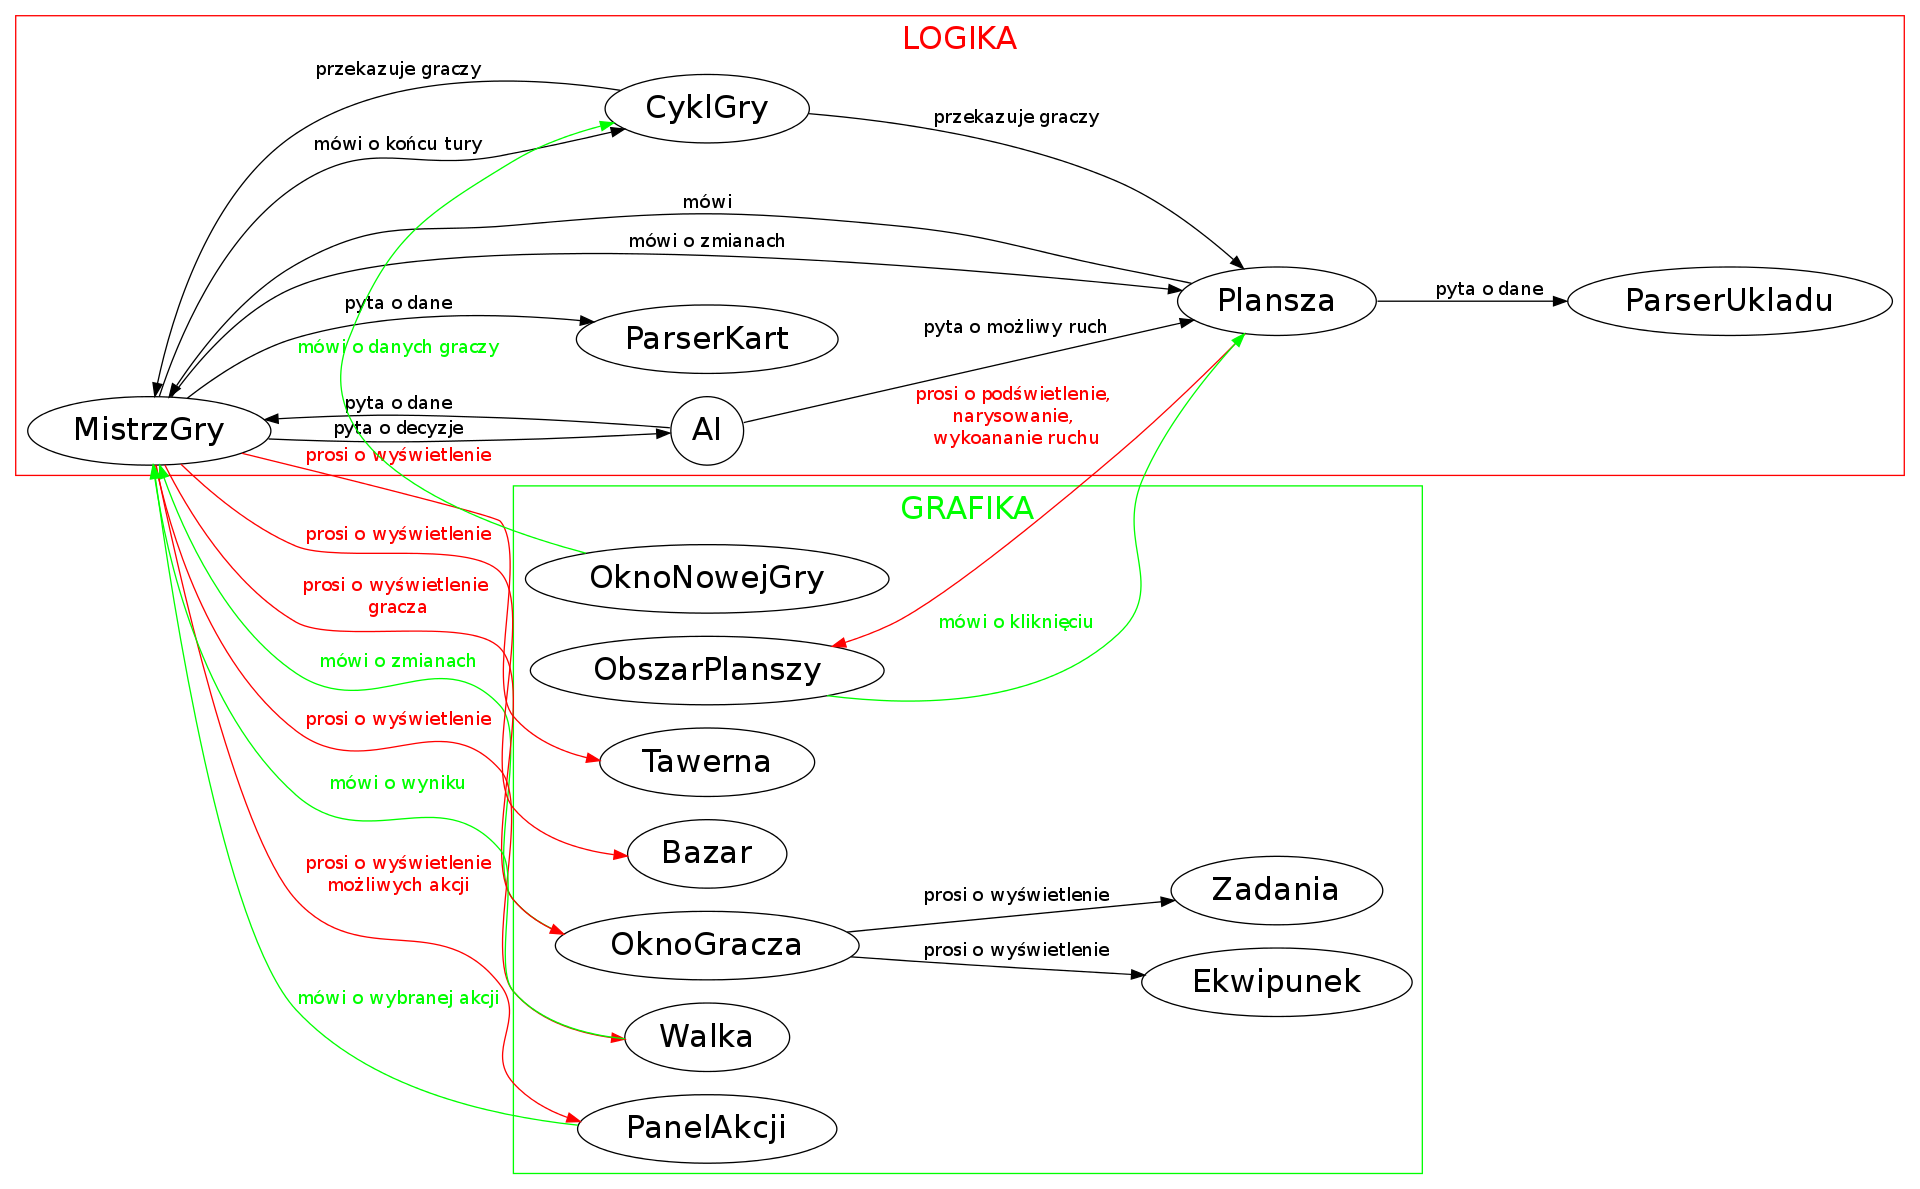
\includegraphics[scale=0.24]{klasy.png}

\caption{Graf modułów projektu z uwzględnieniem podziału na warstwę graficzną i logiczną.} 

\label{Klasy}

\end{figure}

\noindent\textbf{Postać plików na dysku:}

\textbf{Format zapisu przedmiotów:}
\begin{verbatim}
123 baba java patrzy	
\end{verbatim}

\textbf{Format zapisu nagród:}
\begin{verbatim}
123 baba java patrzy	
\end{verbatim}

\textbf{Format zapisów zadań:}
\begin{verbatim}
123 baba java patrzy	
\end{verbatim}

\textbf{Format zapisu przeciwników:}
\begin{verbatim}
123 baba java patrzy	
\end{verbatim}

\newpage

\textbf{Format zapisu planszy:}
\begin{verbatim}
szerokość;wysokość           (2 liczby całkowite dodatnie)

liczba wpisów w legendzie    (liczba całkowite dodatnie)

symbol; nazwa; plik z obrazkiem; czy jest przeciwnik; współczynnik ruchu 
    Format linii legendy:    (tekst(bez spacji);tekst;tekst;1 lub 0; liczba całkowita)

Następnie znajduje się tyle wierszy ile plansza ma wysokości, 
zawierające tyle pól ile szerokości ma plansza.
Pola poodzielane są średnikami i zawierają symbole pól na odpowiednich pozycjach

\end{verbatim}

\begin{figure}[ht]

\centering

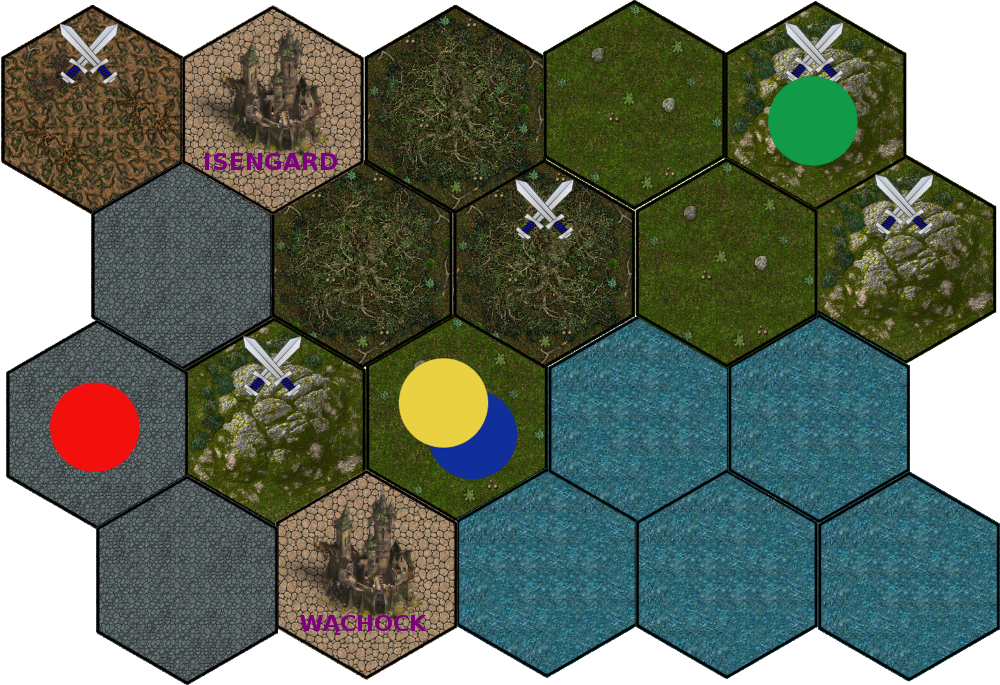
\includegraphics[scale=0.3]{plansza.png}

\caption{Przykładowa plansza.} 

\label{Klasy}

\end{figure}

Zawartość pliku z ustawieniem dla powyższej planszy
\begin{verbatim}
5;4
9
B;;bagno.png;1;3
1;ISENGARD;zamek.png;0;0
l;;las.png;0;2
L;;las.png;1;2
d;;dolina.png;0;1
G;;gora.png;1;2
a;;droga.png;0;1
2;WĄCHOCK;zamek.png;0;0
w;;woda.png;0;2
B;1;l;d;G
 a;l;l;d;G
a;G;d;w;w
 a;2;w;w;w	
\end{verbatim}

\end{document}
